% !TEX TS-program = lualatex
% !TEX encoding = UTF-8 Unicode

% This is a simple template for a LaTeX document using the "article" class.
% See "book", "report", "letter" for other types of document.

\documentclass[10pt, twocolumn]{article} % use larger type; default would be 10pt

\usepackage[utf8]{inputenc} % set input encoding (not needed with XeLaTeX)
\usepackage{fontspec}
\setmainfont{Georgia}
\setsansfont{Georgia}
\setmonofont{Georgia}
%\usepackage[none]{hyphenat}
\usepackage{hyphenat}

%%% Examples of Article customizations
% These packages are optional, depending whether you want the features they provide.
% See the LaTeX Companion or other references for full information.

%%% PAGE DIMENSIONS
\usepackage{geometry} % to change the page dimensions
\geometry{a4paper, left=17.5mm, right=17.5mm, textwidth=85mm,columnsep=5mm, top=17.5mm}
\setlength{\parindent}{0pt}
% or letterpaper (US) or a5paper or....
% \geometry{margin=2in} % for example, change the margins to 2 inches all round
% \geometry{landscape} % set up the page for landscape
%   read geometry.pdf for detailed page layout information

\usepackage{subcaption}
\usepackage{graphicx} % support the \includegraphics command and options

\usepackage[parfill]{parskip} % Activate to begin paragraphs with an empty line rather than an indent

%%% PACKAGES
\usepackage{booktabs} % for much better looking tables
\usepackage{array} % for better arrays (eg matrices) in maths
\usepackage{paralist} % very flexible & customisable lists (eg. enumerate/itemize, etc.)
\usepackage{verbatim} % adds environment for commenting out blocks of text & for better verbatim
%\usepackage{subfig} % make it possible to include more than one captioned figure/table in a single float
\usepackage{amsmath}
% These packages are all incorporated in the memoir class to one degree or another...
\usepackage{lipsum}
%\usepackage{caption}
\usepackage{listings}

%%% HEADERS & FOOTERS
\usepackage{fancyhdr} % This should be set AFTER setting up the page geometry
\pagestyle{fancy} % options: empty , plain , fancy
\renewcommand{\headrulewidth}{0pt} % customise the layout...
\lhead{}\chead{}\rhead{}
\lfoot{}\cfoot{\thepage}\rfoot{}

%%% SECTION TITLE APPEARANCE
%\usepackage{sectsty}
%\allsectionsfont{\sffamily\mdseries\upshape} % (See the fntguide.pdf for font help)
% (This matches ConTeXt defaults)

%%% ToC (table of contents) APPEARANCE
\usepackage[nottoc,notlof,notlot]{tocbibind} % Put the bibliography in the ToC
\usepackage[titles,subfigure]{tocloft} % Alter the style of the Table of Contents
\renewcommand{\cftsecfont}{\rmfamily\mdseries\upshape}
\renewcommand{\cftsecpagefont}{\rmfamily\mdseries\upshape} % No bold!
\usepackage{authblk}

\usepackage{float}

%%% END Article customizations

%%% The "real" document content comes below...

\title{\textbf{Title}}
\author{Candidate Number: 24669}
\affil{Department of Physics, University of Bath, Bath BA2 7AY, United Kingdom}
%\date{} % Activate to display a given date or no date (if empty),
         % otherwise the current date is printed 

\begin{document}
\twocolumn[
 \begin{@twocolumnfalse}
\maketitle
\begin{abstract}
  Diffusion limited aggregation (DLA) clusters are branching fractal objects which arise from the adhesion of random-walking particles. A fractal is an object with fractal dimension, that is its uniform mass density grows to a non-integer power of its linear size. This report examines the fractal dimension of a DLA cluster generated from an initial 'seed' particle (Eden model) and the effects of a random chance of particle adherence on the dimension of the brownian tree. DLA simulations are common in modeling of physical and biological processes such as in coagulated metal aeorosols and the growth of plants. We have determined the fractal dimension of an eden model brownian tree to be 1.72. this allows for better estimates of the density of x objects in y processes.

\bigskip
\end{abstract}
\end{@twocolumnfalse}
]
\medskip

\section*{Introduction}
  Diffusion limited aggregation (DLA) systems have been used to model a variety of physical processes, including...

  DLA models produce brownian trees by adhering random-walking (brownian motion) particles to one another from some initial conditions. A common initial condition and the one that we examine in this report is a single initial particle (Eden model) from which the diffuse particles attach after random walking to the structure from a starting radius.

In our model of the orbit of Hyperion, we employ a two dimensional description of orbit derived from Newtonian mechanics\cite{Newtonian_orbit}, and a correction to include angle of orientation and corresponding angular frequency $(\theta(t), \omega(t))$. This results in a set of six coupled ODEs with corresponding initial conditions, in particular, we will examine the effects of taking different initial conditions of rotational state $(\theta(0),\omega(0))$ on the rotation over many orbits by solving the initial value problem numerically by Runge-Kutta-Fehlberg 45 (rkf45) approximation which is accurate to 5th order. To examine the results a Poincar\'e section of $\omega / \omega_H$ against $\theta$ is taken, where $\omega_H$ is the angular frequency of the orbit of Hyperion about Saturn.

\section*{DLA algorithm and simulation}

\subsection*{Brownian trees}

The model for position and velocity of Hyperions orbit follows directly from Newtonian mechanics, we limit the motion to the x-y plane. The position ($x_H, y_H$) and velocity ($vx_H, vy_H$) of Hyperion are described by the four coupled ODEs

\begin{gather}
\label{position_ODEs}
  \frac{d x_{H}}{d t}=v x_{H},\quad \frac{d y_{H}}{d t}=v y_{H},\\
  \frac{d v x_{H}}{d t}=-\frac{G M x_{H}}{\left(x_{H}^{2}+y_{H}^{2}\right)^{3 / 2}}, \frac{d v y_{H}}{d t}=-\frac{G M y_{H}}{\left(x_{H}^{2}+y_{H}^{2}\right)^{3 / 2}},
\end{gather}

where $M = M_\text{Sat} + M_H$ with $M_\text{Sat} = 5.6832 \times 10^{26}$ kg and $M_H = 5.5855 \times 10^{18}$ kg the masses of Saturn and Hyperion respectively. $G = 6.67408 \times 10^{-11}$ Nm$^2$kg$^{-2}$ is the gravitational constant. For an orbit of eccentricity $e = 0.232$ these ODEs are paired with initial conditions

\begin{gather}
\label{position_ICs}
  x_H(0) = a(1-e), \quad y_H(0) = 0,\\
  vx_H(0) = 0, \quad vy_H(0) = \sqrt{\frac{GM(1+e)}{a(1-e)}},
\end{gather}

where $a = 1.501 \times 10^9$ m is the semi-major axis of orbit. These initial conditions ensure an elliptic orbit clockwise in x-y starting at perihelion. From Keplar's laws we find the period of the orbit $T_H = \sqrt{4\pi^2a^3/GM} = 1.876\times10^6$ s from which we can determine the angular frequency $\omega_H = 2\pi/T_H = 3.349\times10^{-6}$ rad s$^{-1}$.

This is a simple classical model of orbit that doesn't consider the rotation of Hyperion, we can quantify error in our numerical solution by considering the difference in position and velocity at perihelion after $n$ orbits, which should stay constant. Analysis of this difference shows that after $n=100$ orbits the difference in magnitude of position and velocity are ~10$^{-6} \times$ the magnitudes of our initial conditions. We will take this error as negligible as in our analysis we don't generate data for greater than 100 orbits. If a very large number of orbits were modelled this error could be far greater.

\begin{figure}[tb!]
\centering
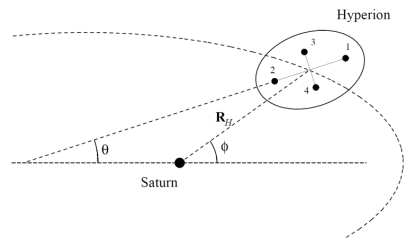
\includegraphics[width=0.95\columnwidth]{hyperion_orbit_diagram.png}
  \caption{Diagram of the orbit of Hyperion in the x-y plane with angle $\phi$ to the line of periapse (major axis) and radius $R_H$. Shown are the four equal masses from which the axes of moments of inertia $I_1, I_2$ are determined. The orientation $\theta$ of Hyperion is defined as the angle made between the axis of smallest moment of inertia and the line of periapse. This diagram is taken from the project assignment sheet by S. Crampin \cite{Crampin}.}
\label{orientation_diagram}
\end{figure}

\subsection*{Asphericity and rotation}

The model is extended to consider the asphericity of Hyperion. Because of its asphericity it we can define its orientation $\theta$. Our model is simplified by restriction of motion the x-y plane of orbit, so its spin axis is in the $z$, normal ot the orbit plane, we also take this to be the axis with the largest mass moment of inertia $I_3$. The orientation of Hyperion $\theta$ is then defined to be the angle between its smallest moment of inertia and the line of periapse of its orbit, this is more clearly shown in FIG. \ref{orientation_diagram}.

The dynamics of the orientation $\theta$ are found by substituting the actual mass distribution with four equal masses in the x-y plane such that the lines of seperation between these masses align with the axes of moments of inertia $I_1, I_2$.

We define the asphericity factor of Hyperion to be $\beta = \sqrt{3(I_2 - I_1)/I_3} = 0.89$. By examining the contributions to torque from our model we can retrieve an expression for the net torque $T$ about the axis of rotation aligned with $z$. This equivalent to the change in angular momentum $T = I_3 \frac{d^2\theta}{dt^2}$, and hence

\begin{equation}
    \frac{T}{I_3} = \frac{d^2\theta}{dt^2} = - \frac{GM_{sat}\beta^2}{2R_{H}^{3}}\sin 2(\theta - \phi)
\end{equation}

Where $\phi$ is the angle of the orbit around Saturn against the line of periapse and $R_H = \sqrt{x_H^2 + y_H^2}$ is the radius of orbit. We then use two coupled first order ODEs to describe the rotation of Hyperion

\begin{equation}
  \label{angle_ODEs}
  \frac{d\theta}{dt} = \omega, \quad \frac{d\omega}{dt} = - \frac{GM_{sat}\beta^2}{2R_{H}^{3}}\sin 2(\theta - \phi). 
\end{equation}

\begin{figure}[tb!]
\centering
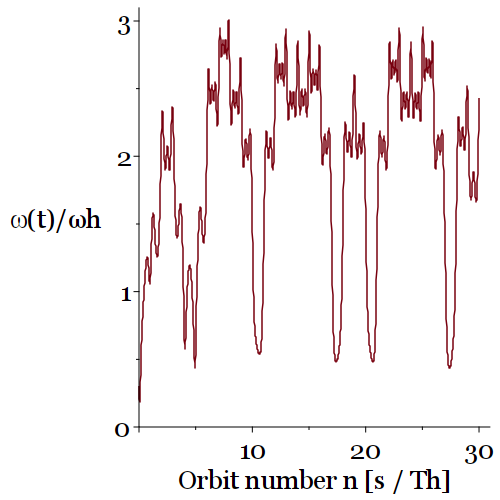
\includegraphics[width=0.95\columnwidth]{angular_freq_chaos.png}
  \caption{Plot of angular frequency $\omega(t)$ against time (number of orbits $T_H$) of Hyperion for initial conditions $\omega(0) = 0.3\omega_H \theta(0) = \pi/7$ where $\omega_H$ is the angular frequency of Hyperions orbit about Saturn. There is chaotic behaviour with some seemingly recurring patterns, these can be interpreted as states of rotation that are more likely to occur in this chaotic system.}
\label{angular_freq_chaos}
\end{figure}

The initial conditions of $\theta$ and $\omega$ are not known and will serve as our independent variables in further analysis.

A plot of $\omega(t)$ against $t$ for some initial conditions $\omega(0) = 0.3\omega_H \theta(0) = \frac{\pi}{7}$ seen in FIG. \ref{angular_freq_chaos} displays some chaotic behaviour, that is, random behaviour in a deterministic system. Because of the chaotic nature of this motion, it is not possible to distinguish error from chaos in any measurements of $\theta$ and $\omega$.

\section*{Poincar\'e section}

\begin{figure}[tb!]
  \centering
  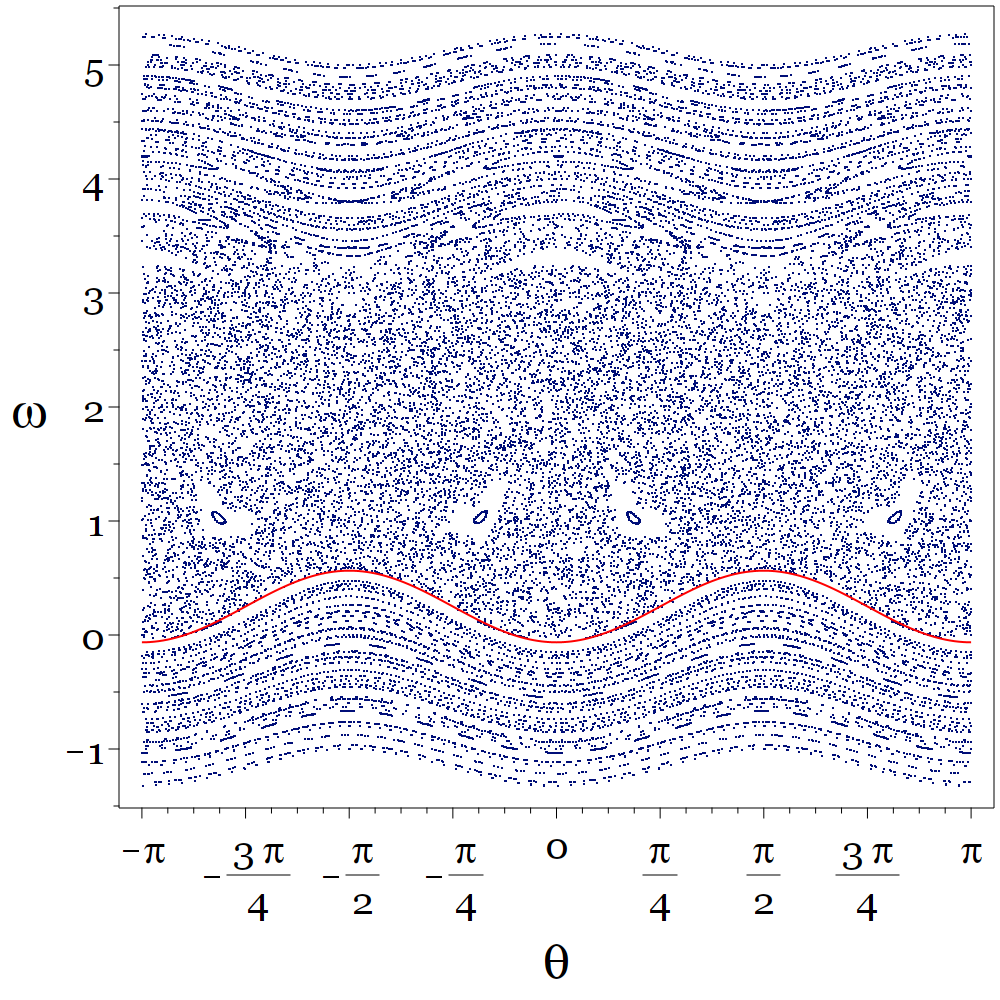
\includegraphics[width=0.95\columnwidth]{poincare_section.png}
  \caption{Poincar\'e section plot of $\omega / \omega_H$ against $\theta$ at $t = nT_H$ for $n$ orbits in the interval $[0,50]$ with initial conditions $\theta(0) \in [0, 2 \pi], \omega(0) \in [-1, 5 \omega_H]$ with intervals of $0.1 \pi$ and $0.3 \omega_H$ respectively (33201 points). The majority of the plot is dominated by a large 'chaotic sea' bounded by periodic patterns of states $\omega = A \mathrm{cos}(2\theta)+B$ for constants $a,b$ (highlighted in red). There are also notable 'islands' of states in the chaotic sea where there are voids with a distinct lack of rotational states a dense region of states within.}
\label{poincare_section}
\end{figure}


\begin{figure}[tb!]
  \centering
  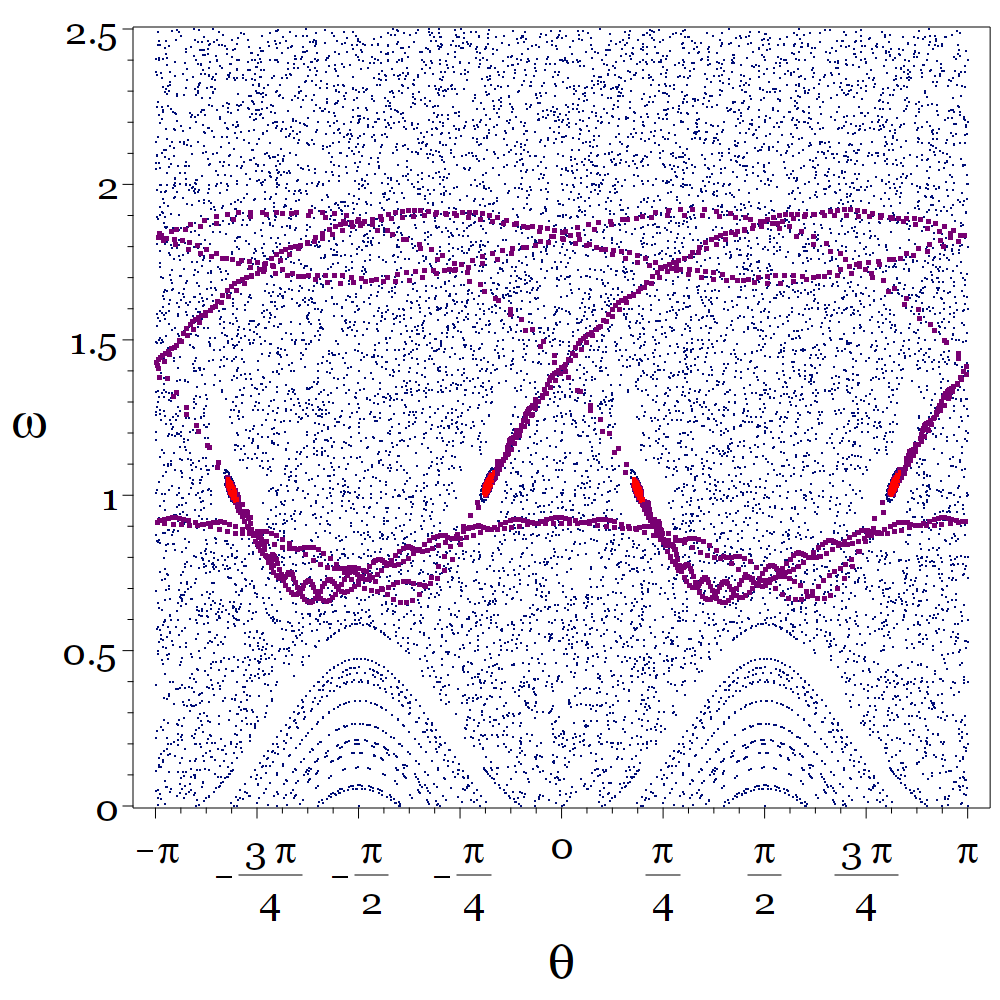
\includegraphics[width=0.95\columnwidth]{unstable_islands.png}
  \caption{Poincar\'e section plot for initial conditions $\theta(0) = -13\pi/16, -3\pi/16, 3\pi/16, 13\pi/16$, $\omega(0) = \omega_H$ and $n = 100$ (404 points, red). The states remain firmly in the bounds of the 'islands' in the chaotic sea. However for initial condition $\theta(0) = -13\pi/16, \omega(0) = \omega_H$ starting in just one island, over many more orbits $n = 1500$ (1501 points, purple) the orbit evolves to reveal a periodic unstable nonsynchronous set of states within the chaotic region (FIG \ref{poincare_section}, blue).}
  \label{poincare_islands}
\end{figure}

\begin{figure*}[th!]
  \centering
  \begin{subfigure}[t]{.45\textwidth}
    \centering
    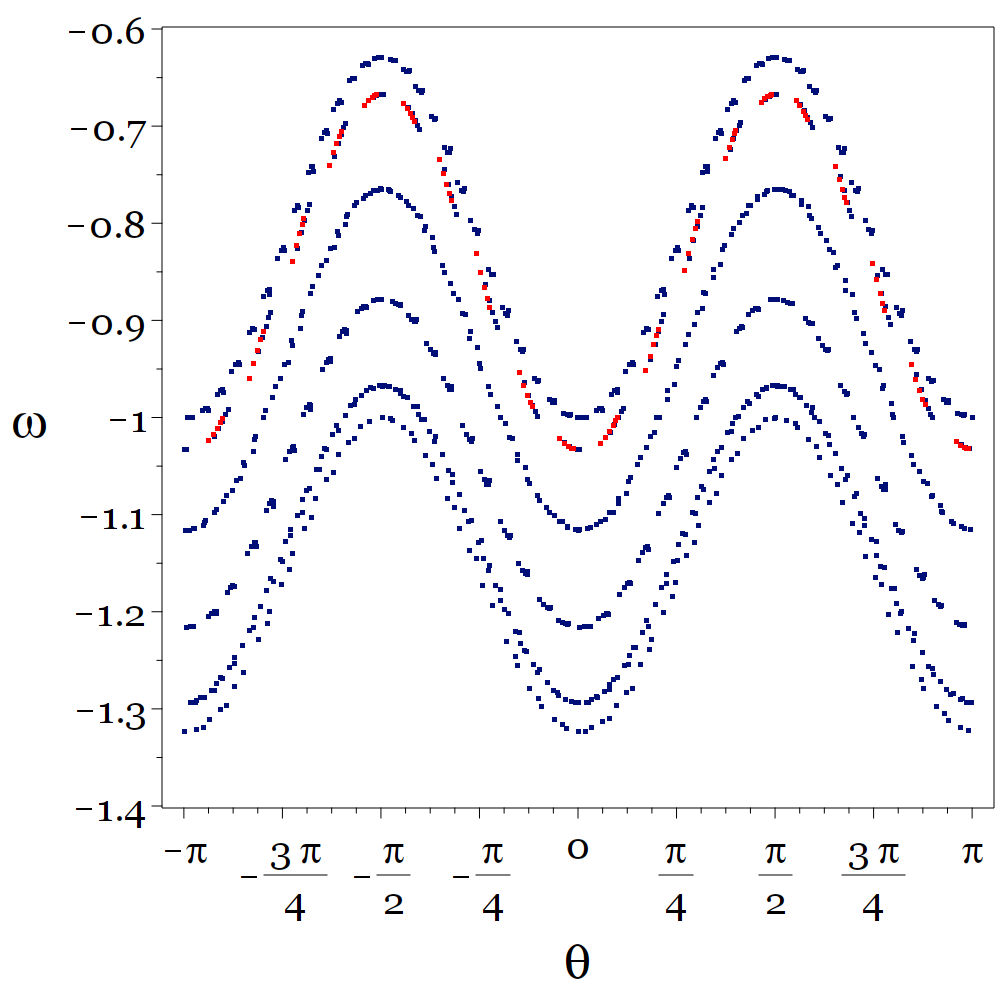
\includegraphics[width=0.95\textwidth]{poincare_nearby_bands.png}
    \caption{Poincar\'e section plot for initial conditions $\theta(0) \in [0, \pi]$ with interval $\pi/10$, $\omega(0) = -\omega_H$ and $n = 100$ (1111 points). There are six distinct 'bands' of rotational states of form $A \mathrm{cos}(2\theta) + B$. Highlighted in red is the band from initial condition $\theta(0) = \pi/10$}
    \label{poincare_bands}
  \end{subfigure}
  \hfill
  \begin{subfigure}[t]{.45\textwidth}
    \centering
    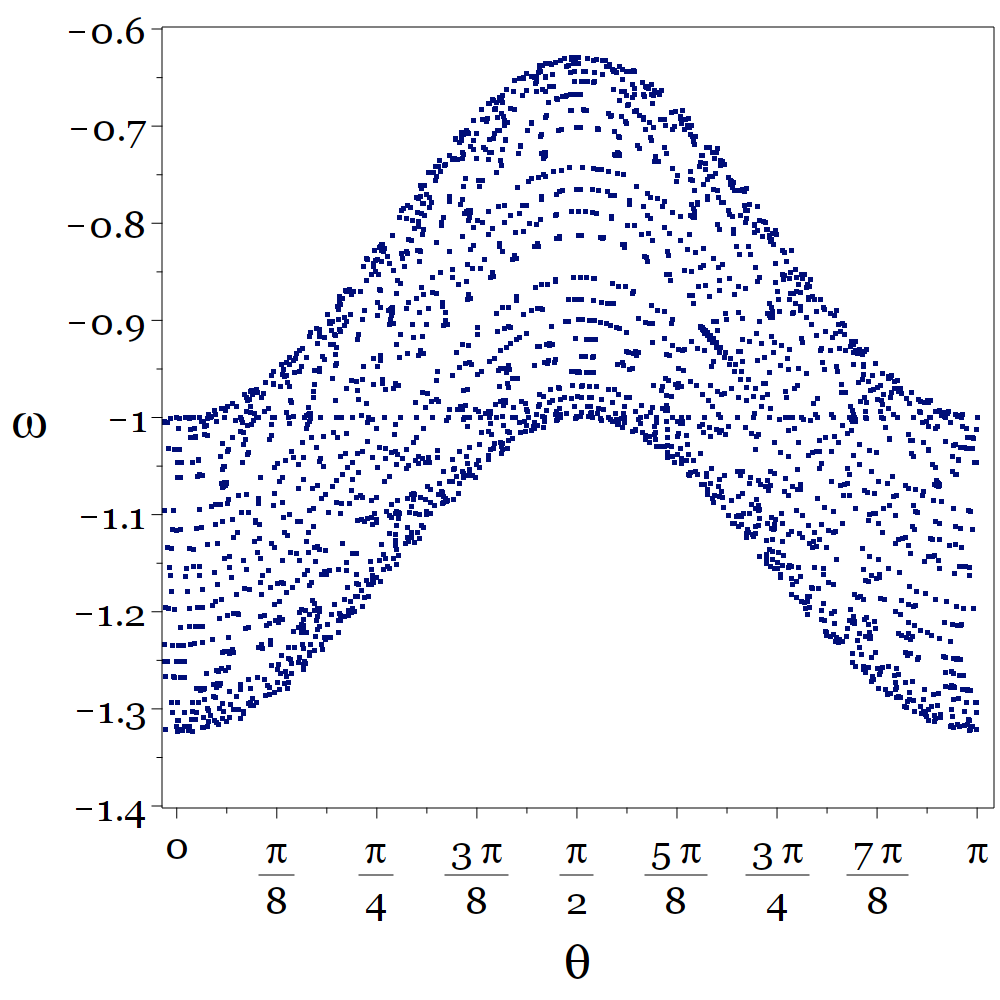
\includegraphics[width=0.95\textwidth]{poincare_nearby_bands_more_samples.png}
    \caption{Poincar\'e section plot restricted to $\theta = [0, \pi]$ for initial conditions $\theta(0) \in [0, \pi]$ with interval $\pi/50$, $\omega(0) = -\omega_H$ and $n = 100$ (5151 points). When more samples are taken the bands become less distinct.}
    \label{poincare_bands_more_samples}
  \end{subfigure}
  \label{poincare_detail_graphs}
  \caption{Poincar\'e section plots of $\omega(t) / \omega_H$ against $\theta(t)$ at $t = nT_H$ for varying initial conditions $\omega(0), \theta(0)$ and over number of orbits $n$. Initial conditions are selected to highlight regions of interest.}
\end{figure*}

To gain further insight on this chaotic behavior in FIG \ref{poincare_section} we take a Poincar\'e section of $\omega(t) / \omega_H$ against $\theta(t)$ modulo $2\pi$ at perihelion $t = nT_H$ for $n \in \mathbb{N}$. The Poincar\'e section is taken with $n = 1 \cdots 100$ orbits and initial conditions $\theta(0) \in [0, 2 \pi], \omega(0) \in [-1, 5 \omega_H]$ with intervals of $0.1 \pi$ and $0.2 \omega_H$ respectively for a total of 33,201 sampled points. FIG \ref{poincare_section} and the procedure \verb+poincare()+ that generates these points are detailed in the appendix. Qualitatively, we observe a large 'chaotic sea' of rotational states bounded by periodic sets of states $\omega(t) = A \mathrm{cos}(2\theta) + B$ for constants $A, B$. These periodic sets of states continue outside of the chaotic sea in a discrete way, forming 'bands' of rotational states. Finally there are distinct 'islands' in the chaotic sea around $\omega = 0$ and $\theta = -13\pi/16, -3\pi/16, 3\pi/16, 13\pi/16$ where at each island there is a small dense region of states within a surrounding empty region.

To further examine these periodic patterns in FIG \ref{poincare_detail_graphs} Poincar\'e sections are taken with initial conditions in these regions of interest. Firstly, in FIG \ref{unstable_islands} with initial conditions $\theta(0) = -13\pi/16, -3\pi/16, 3\pi/16, 13\pi/16, \omega(0) = \omega_H$ around the islands at we see four distinct sets of states with the same orientation $\theta$ over a very low range of angular frequency $\Delta\omega \approx 0.08\omega_H$. In FIG \ref{unstable_islands} a plot is taken with just one initial condition at the island corresponding to $\theta(0) = -13\pi/16$ over a large number of orbits $n = 1500$, we reveal an unstable periodic set of states inside the chaotic region. This set of states visits the four other islands after several orbits. It is likely that this corresponds to one of the nonsynchronous $p$ states inside the chaotic region discussed by J. Wisdom \textit{et al}. However due to the larger number of orbits measured, the error in position and velocity could be large enough to effect the states seen, especially due to their high dependence on initial conditions.

In FIG \ref{poincare_bands} when initial conditions are taken across $\omega(0) = -\omega_H$ the result is a set of six distict 'bands' of rotational states. The primary similarity between these bands is that they have the form $A \mathrm{cos}(2\theta) + B$, and that they all cross the line $\omega(\theta)=-\omega_H$, with the highest and lowest bands having their minima and maxima respectively almost exactly at $-\omega_H$. This suggests that states outside of the chaotic region are more stable and generally stick to a set range of angular frequencies.

We take a larger sample of points from more initial conditions $\theta(0) \in [0, \pi]$ with interval $\pi/50$ and $\omega(0)=-\omega_H$ in FIG \ref{poincare_bands_more_samples}. We see that the region bounded by the upper and lower bands in FIG \ref{poincare_bands} is now full of many sinusoidal patterns, however they are much harder to distinguish, and states near the upper and lower bounds begin to look looks chaotic. Interestingly at $\theta \approx 21\pi/32, \omega \approx -0.95\omega_H$ there is a particularily dense region of states. The fact that chaos can be found in the fine strucure of a Poincar\'e plot outside of the chaotic sea is supported by the literature \cite{}

This is further supported by additional computations excluded from this written report but that are accessible in the accompanying worksheet that show for a single initial condition state, for small $n ~ 100$ a band can be isolated and is stable, however as the orbit evolves to say, $n ~ 10000$ it becomes chaotic, but is still bounded in $\omega$ to the same region as the isolated band. This computation of course may be heavily effected by error in computing values for such a large $n$.

\section*{Comparison with a less eccentric orbit}
To develop our insight on the effects of orbit eccentricity $e$ and the asphericity $\beta$ on the rotational states of an orbit we construct a toy model which substitutes the eccentricity of orbit and apshericity Hyperion to that of the Martian moons Deimos and Phobos. All other parameters, in particular the masses $M_\text{Sat}, M_H$ involved and the semi-major axis $a$ are preserved.

mars graphs discussion here

\section*{Conclusion}

begin conclusion

poincare results

mars results

End conclusion

\section*{Acknowledgements}
We would like to acknowledge the contributions of Dr S. Crampin for his code and resources on which this model is based, and N. Roberts for providing the latex template used in the creation of this report.

%%%References
\bibliographystyle{ieeetr}
%bibliographystyle{bathx}
\bibliography{refs}

\clearpage

\section*{Appendix}
The numerical... was done using maple

Try to make this single width

Eqns, ICs
\begin{lstlisting}
Eqns := {diff(vxh(t), t) = -G*M*xh(t)/Rh(t)^3,
          diff(vyh(t), t) = -G*M*yh(t)/Rh(t)^3,
          diff(xh(t), t) = vxh(t),
          diff(yh(t), t) = vyh(t)};

ICs := {vxh(0) = 0,
        vyh(0) = sqrt(G*M*(1 + e)/(a*(1 - e))),
        xh(0) = a*(1 - e),
        yh(0) = 0};
\end{lstlisting}

with rotation TIDY THIS
\begin{lstlisting}
Eqns_rotation := Eqns union {diff(omega(t), t) = -G*M_sat*beta^2*(xh(t)*sin(theta(t)) - yh(t)*cos(theta(t)))*(xh(t)*cos(theta(t)) + yh(t)*sin(theta(t)))/Rh(t)^5,
diff(theta(t), t) = omega(t)};
\end{lstlisting}

Code developed for use in taking Poincar\'e sections: The \textit{poincare()} procedure, written in maple, takes inputs for \textit{theta0, omega0|} the initial conditions for rotation and \textit{n} the number of orbits to generate data for. \textit{theta0} and \textit{omega0} should be given as lists of values, for a single intitial condition lists of one item can be passed to the procedure.\textit{poincare()} will then find each state $(\theta(t) \text{mod} 2\pi, \omega(t)/\omega_H)$ where $t = nT_H$ for $n$ from 0 to $n$ at every combination of initial conditions $\theta(0) = \text{theta0}$ and $\omega(0) = \text{omega0}$ it recieves. The resulting data is output as an array of touples.

\begin{lstlisting}
poincare := proc(theta0::list, omega0::list, n::nonnegint)
  local data, local_ICs, soln, omeg, thet, i, j, k;
  global wh, Eqns_rotation, ICs, ICs_rotation;
  data := [];
  for i in theta0 do 
    for j in omega0 do 
      local_ICs := ICs union {omega(0) = j, theta(0) = i};
      soln := dsolve({Eqns_rotation[], local_ICs[]}, numeric, maxfun = -1, range = 0 .. (n + 1)*Th);
      for k from 0 to n do 
        omeg := rhs(soln(k*Th)[2])/wh;
        thet := frem(rhs(soln(k . Th)[3]), evalf(2*Pi));
        data := [op(data), [thet, omeg]];
      end do;
    end do;
  end do;
  return data;
end proc:
\end{lstlisting}

\clearpage

\begin{figure*}[t]
\centering
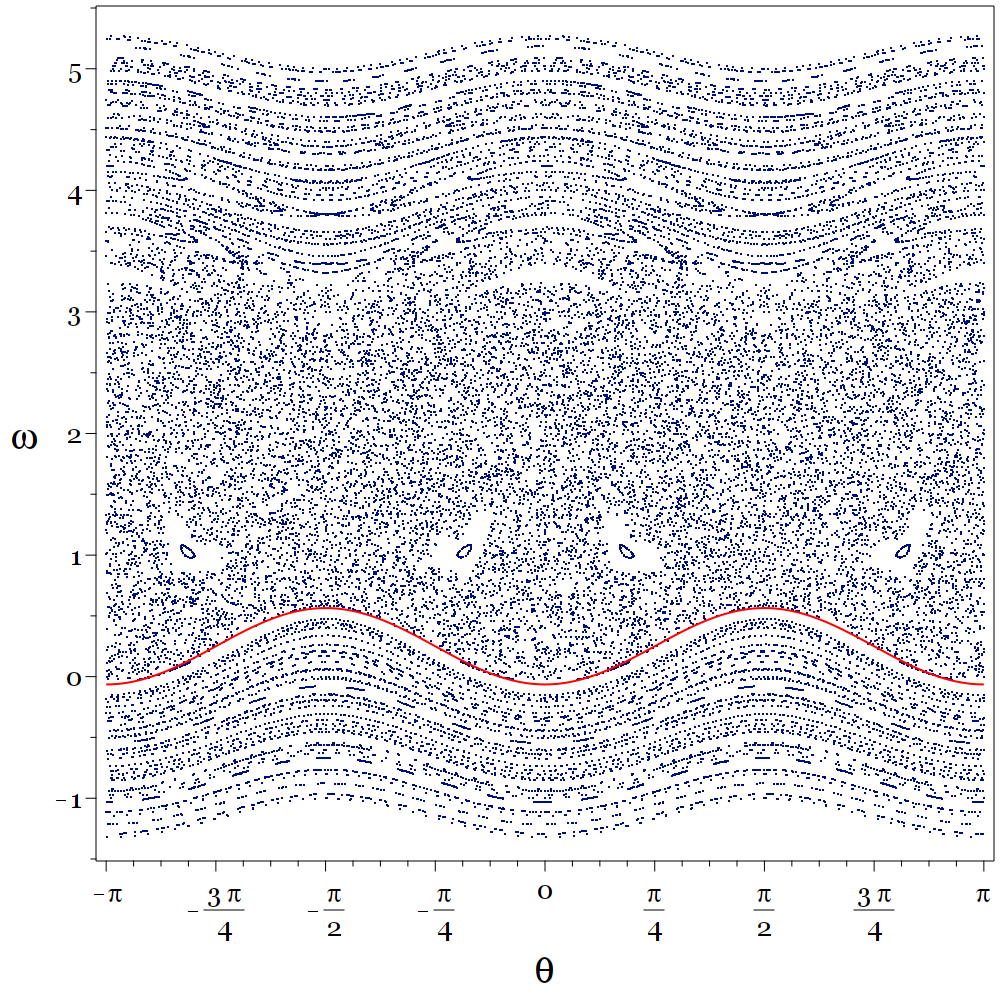
\includegraphics[width=0.95\textwidth]{poincare_section_large.png}
  \caption{Poincar\'e section plot of $\omega / \omega_H$ against $\theta$ at $t = nT_H$ for $n$ orbits in the interval $[0,50]$ with initial conditions $\theta(0) \in [0, 2 \pi], \omega(0) \in [-1, 5 \omega_H]$ with intervals of $0.1 \pi$ and $0.3 \omega_H$ respectively (33201 points). The majority of the plot is dominated by a large 'chaotic sea' bounded by periodic patterns of states $\omega = A \mathrm{cos}(2\theta)+B$ for constants $a,b$ (highlighted in red). There are also notable 'islands' of states in the chaotic sea where there are voids with a distinct lack of rotational states a dense region of states within.}
\label{poincare_section_large}
\end{figure*}

\end{document}
